\documentclass{article}
\setlength{\parskip}{0pt} % esp. entre parrafos
\setlength{\parindent}{20pt} % esp. al inicio de un parrafo
\usepackage{amsmath} % mates
\usepackage{listings}
\usepackage{xcolor}
\usepackage[sort&compress,numbers]{natbib} % referencias
\usepackage{url} % que las URLs se vean lindas
\usepackage[top=10mm,left=20mm,right=20mm,bottom=25mm]{geometry} % \textbf{\textbf{}}margenes
\usepackage{hyperref} % ligas de URLs
\usepackage{graphicx} % poner figuras
\usepackage{caption}
\usepackage{subcaption}
\usepackage[spanish]{babel} % otros idiomas
\hypersetup{
    colorlinks=true,
    linkcolor=blue,
    filecolor=blue,      
    urlcolor=blue,
}
\renewcommand{\lstlistingname}{C\'odigo}
\definecolor{codegreen}{rgb}{0,0.6,0}
\definecolor{codegray}{rgb}{0.5,0.5,0.5}
\definecolor{codepurple}{rgb}{0.58,0,0.82}
\definecolor{backcolour}{rgb}{0.95,0.95,0.92}
\lstdefinestyle{mystyle}{
    backgroundcolor=\color{backcolour},   
    commentstyle=\color{codegreen},
    keywordstyle=\color{magenta},
    numberstyle=\tiny\color{codegray},
    stringstyle=\color{codepurple},
    basicstyle=\ttfamily\footnotesize,
    breakatwhitespace=false,         
    breaklines=true,                 
    keepspaces=true,                 
    numbers=left,                    
    numbersep=5pt,                  
    showspaces=false,                
    showstringspaces=false,
    showtabs=false,                  
    tabsize=2
}
\lstset{style=mystyle}

\title{Reporte 6:\\Sistema Multiagente}
\author{Jorge Torres}
\date{\today}

\begin{document}

\maketitle

\section{Objetivo}
En esta pr\'actica se implementa un sistema multiagente aplicado en epidemiolog\'ia a trav\'es del modelo SIR, que consiste en definir tres tipos de agentes: susceptibles, infectados y recuperados. El objetivo es el de analizar el efecto que tiene el contener o reducir la velocidad de movimiento de los agentes infectados, tanto en la magnitud de la epidemia (la altura del pico en la curva del porcentaje de infectados por iteración), como en su velocidad (la iteración en la cual se llega por la primera vez al valor pico).

\section{Desarrollo}
Basando el desarrollo de la pr\'actica en el \href{https://github.com/satuelisa/Simulation/blob/master/MultiAgent/SIR.py}{c\'odigo} desarrollado por E. Schaeffer \cite{elisa1}, en primer lugar, se definen los par\'ametros iniciales con los cuales act\'ua el sistema, como se observa en el c\'odigo \ref{codigo1}. Estos se conforman por 1) el largo de cada lado del sistema, \texttt{l}, 2) la cantidad de agentes que se crean, \texttt{n}, 3) la probabilidad inicial de infectados, \texttt{pi}, 4) la probabilidad de que cada agente infectado se recupere, \texttt{pr}, 5) la velocidad inicial de los agentes, \texttt{v}, 6) el umbral de cercan\'ia para considerar una infecci\'on, \texttt{r}, 7) la cantidad de pasos que hacen los agentes, \texttt{tmax}, y 8) la cantidad de veces que se repite el experimento, \texttt{runs}. El \href{https://github.com/FeroxDeitas/Simulacion-Nano/blob/main/Tareas/P6/epidemia_r.py}{desarrollo} completo se puede observar en el repositorio en GitHub de J. Torres \cite{jorge1}

\begin{lstlisting}[caption=Par\'ametros Iniciales, label=codigo1, language=Python]
l = 1.5
n = 50
pi = 0.05
pr = 0.02
v = l / 30
r = 0.1
tmax = 100
runs = 100
\end{lstlisting}

Con la funci\'on \texttt{contagiados()} del c\'odigo \ref{codigo2} se decide qu\'e agentes son los pr\'oximos en infectarse de acuerdo a la probabilidad, $p_c$, descrita en la ecuaci\'on \ref{eq1},

\begin{equation}\label{eq1}
    p_c =
    \begin{cases}
    0\text{,} & \text{si} \ d(i,j) \geq r\text{,}\\
    \frac{r-d}{r}\text{,} & \text{para cualquier otro caso,}
    \end{cases}
\end{equation}
donde $d$ es la distancia euclideana entre un par, $(i,j)$, de agentes y $r$ es el umbral de cercan\'ia.

\begin{lstlisting}[caption=Nuevos Agentes Infectados, label=codigo2, language=Python]
def contagiados():
    for i in range(n):
        a1 = agentes.iloc[i]
        if a1.estado == 'I':
            for j in range(n):
                a2 = agentes.iloc[j]
                if a2.estado == 'S':
                    d = sqrt((a1.x - a2.x)**2 + (a1.y - a2.y)**2)
                    if d < r:
                        if random() < (r - d) / r:
                            contagios[j] = True
    return contagios
\end{lstlisting}

Utilizando el c\'odigo \ref{codigo3}, se crean los agentes, se distribuyen uniformemente a trav\'es del espacio y se decide su estado inicial de infecci\'on utilizando la probabilidad inicial, \texttt{pi}. Adem\'as, para cada agente creado, se decide de manera aleatoria un diferencial de movimiento que representa su velocidad, dado por los t\'erminos \texttt{dx} y \texttt{dy}.

\begin{lstlisting}[caption=Creaci\'on de Agentes, label=codigo3, language=Python]
agentes =  pd.DataFrame()
agentes['x'] = [uniform(0, l) for i in range(n)]
agentes['y'] = [uniform(0, l) for i in range(n)]
agentes['estado'] = ['S' if random() > pi else 'I' for i in range(n)]
agentes['dx'] = [uniform(-v, v) for i in range(n)]
agentes['dy'] = [uniform(-v, v) for i in range(n)]
\end{lstlisting}

Con las l\'ineas del c\'odigo \ref{codigo4} se lleva un conteo de la cantidad de infectados para cada paso iterado, y se manda a llamar a la funci\'on \texttt{contagiados()} del c\'odigo \ref{codigo2} para decidir los nuevos agentes infectados. Si la cantidad de infectados llega a cero, el programa se detiene.

\begin{lstlisting}[caption=Conteo de Infectados, label=codigo4, language=Python]
epidemia = []
    for tiempo in range(tmax):
        conteos = agentes.estado.value_counts()
        infectados = conteos.get('I', 0)
        epidemia.append(infectados)
        contagios = [False for i in range(n)]
        if infectados == 0:
            break
        contagios = contagiados()
\end{lstlisting}

En seguida, se decide si un agente cambia de estado a infectado (por medio de la funci\'on \texttt{contagiados()}, descrita previamente), o a recuperado por medio de la probabilidad de recuperaci\'on, \texttt{pr}. En el c\'odigo \ref{codigo5} se observan \'estas funciones.

\begin{lstlisting}[caption=Decisi\'on de Agentes Infectados y Recuperados, label=codigo5, language=Python]
        for i in range(n):
            a = agentes.iloc[i]
            if contagios[i]:
                agentes.at[i, 'estado'] = 'I'
            elif a.estado == 'I':
                if random() < pr:
                    agentes.at[i, 'estado'] = 'R'
\end{lstlisting}

Por \'ultimo, se trasladan todos los agentes a su nueva posici\'on dada por los diferenciales \texttt{dx} y \texttt{dy}, establecidos en el c\'odigo \ref{codigo3}. Las l\'ineas \texttt{3} a \texttt{6} simplemente establecen que los agentes que lleguen a un l\'imite del plano reaparecen en el l\'imite opuesto, con la misma velocidad y direcci\'on. Con las l\'ineas \texttt{9} y \texttt{10} se crea una lista de la cantidad m\'axima de infectados y la iteraci\'on en la que se lleg\'o por primera vez a esa cantidad, para todas las repeticiones del experimento. Esto se observa en el c\'odigo \ref{codigo6}.

\begin{lstlisting}[caption=Movimiento de los Agentes, label=codigo6, language=Python]
        x = a.x + a.dx
        y = a.y + a.dy
        x = x if x < l else x - l
        y = y if y < l else y - l
        x = x if x > 0 else x + l
        y = y if y > 0 else y + l
        agentes.at[i, 'x'] = x
        agentes.at[i, 'y'] = y
    maximos['Maximos Infectados'].append(max(epidemia))
    maximos['Posicion'].append(epidemia.index(max(epidemia)) + 1)
\end{lstlisting}

\subsection{Reducci\'on de Velocidad de Agentes Infectados}

Para hacer una comparaci\'on entre el modelo epidemiol\'ogico con agentes infectados a velocidad normal y uno en donde \'estos reducen su velocidad a la mitad, se tienen que realizar algunas modificaciones. Las l\'ineas \texttt{5} y \texttt{6} del c\'odigo \ref{codigo3} se modifican para reducir la velocidad de los agentes inicialmente infectados a la mitad, como se observa en el c\'odigo \ref{codigo7}.

\begin{lstlisting}[caption=Modificaci\'on del C\'odigo 3, label=codigo7, language=Python]
agentes['dx'] = [uniform(-v/2, v/2) if  agentes.at[i, 'estado'] == 'I'\
                 else uniform(-v, v) for i in range(n)]
agentes['dy'] = [uniform(-v/2, v/2) if  agentes.at[i, 'estado'] == 'I'\
                 else uniform(-v, v) for i in range(n)]
\end{lstlisting}

Por otro lado, al c\'odigo \ref{codigo5} se agregan dos l\'ineas para reducir la velocidad de los nuevos agentes infectados, de tal manera que resulta en el c\'odigo \ref{codigo8}.

\begin{lstlisting}[caption=Modificaci\'on del C\'odigo 5, label=codigo8, language=Python]
        for i in range(n):
            a = agentes.iloc[i]
            if contagios[i]:
                agentes.at[i, 'dx'] /= 2
                agentes.at[1, 'dy'] /= 2
                agentes.at[i, 'estado'] = 'I'
            elif a.estado == 'I':
                if random() < pr:
                    agentes.at[i, 'estado'] = 'R'
\end{lstlisting}

\section{Resultados}

En los diagramas de la figura \ref{epidemias} se puede observar una comparaci\'on entre las distribuciones de los picos de infectados y las iteraci\'ones en que se llega por primera vez a esos picos, para una epidemia con velocidad normal de agentes (figura \ref{fast}) y una en donde los agentes infectados reducen su velocidad a la mitad (figura \ref{slow}).

\begin{figure}[h]
     \begin{subfigure}[b]{0.49\textwidth}
         \centering
         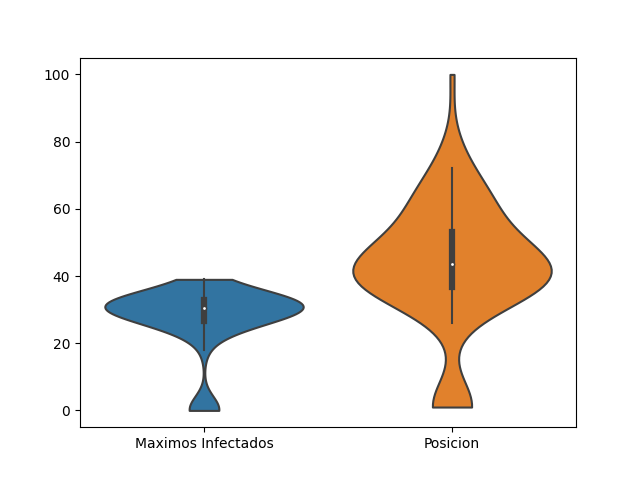
\includegraphics[width=\textwidth]{Fast_Epidemic.png}
         \caption{Distribuci\'on de epidemia a velocidad normal.}
         \label{fast}
     \end{subfigure}
     \begin{subfigure}[b]{0.49\textwidth}
         \centering
         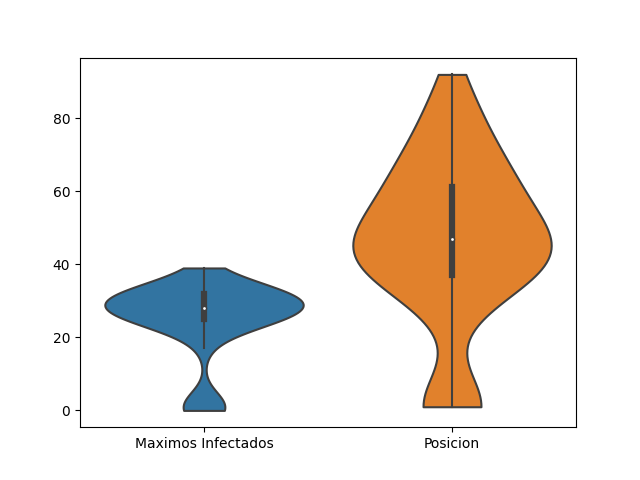
\includegraphics[width=\textwidth]{Slow_Epidemic.png}
         \caption{Distribuci\'on de epidemia con velocidad reducida.}
         \label{slow}
     \end{subfigure}
     \caption{Distribuciones de m\'axima cantidad de infectados y posici\'on del pico para cada tipo de epidemia.}
     \label{epidemias}
\end{figure}

\section{Conclusiones}

Al analizar la comparaci\'on de la figura \ref{epidemias}, se puede observar que, al reducir la velocidad de agentes infectados, no hay una diferencia relevante en cuanto a la m\'axima cantidad de infectados, ambas epidemias llegando a picos de aproximadamente 30. Esto puede deberse a la cantidad limitada de agentes totales y el hecho de que los agentes recuperados ya no pueden infectarse ni propagar la infecci\'on.\\

Por otro lado, s\'i se observa una diferencia significativa en cuanto al comportamiento en el tiempo de la epidemia, observando que la velocidad de infecci\'on se reduce al hacerlo tambi\'en la velocidad de los agentes infectados, propag\'andose m\'as lentamente.

\bibliography{tarea_6}
\bibliographystyle{plainnat}
\end{document}
